% !TeX root = main.tex
\documentclass[12pt]{article}

\usepackage[utf8]{inputenc}
\usepackage[T1]{fontenc}
\usepackage{graphicx}
\usepackage{amsmath}
\usepackage{geometry}
\usepackage{setspace}
\usepackage{lmodern}

\geometry{a4paper, margin=2.5cm}

\title{Interoperabilidade e padronização de conectores de carregamento de veículos elétricos no Brasil: evidências comparativas da Europa e da América Latina}
\author{Valdir Luis de Souza}
\date{\today}
\usepackage{enumitem}
\usepackage{graphicx}
\graphicspath{{figures/}}
\begin{document}

\maketitle

\begin{abstract}
A expansão da mobilidade elétrica depende da disponibilidade, interoperabilidade e padronização da infraestrutura de recarga. No Brasil, a consolidação de padrões tecnológicos para conectores e estações de carregamento influencia diretamente decisões de investimento privado, política industrial e planejamento regulatório. Este artigo analisa a relação entre padronização de conectores, potência instalada e maturidade da infraestrutura de recarga, com foco no Brasil e benchmarking internacional com Alemanha, França, Espanha e México, além de referência institucional à China. A pesquisa utiliza dados secundários obtidos por meio da API do Open Charge Map e bases complementares de literatura e relatórios institucionais. Foram aplicadas estatística descritiva, ANOVA, teste de Tukey e regressão linear múltipla para avaliar o impacto do tipo de conector e do país sobre a potência instalada de recarga. Os resultados indicam predominância do padrão CCS2 e Type 2 no Brasil e na Europa, enquanto o México apresenta maior aderência aos padrões CCS1 e Type 1, associados ao ecossistema norte-americano. A regressão mostrou que o tipo de conector e o país explicam aproximadamente 49,7% da variação da potência instalada, evidenciando que a padronização reflete não apenas escolhas técnicas, mas também alinhamentos geotcnológicos e estruturais. Conclui-se que o Brasil apresenta convergência tecnológica com o modelo europeu, embora ainda possua menor maturidade em potência instalada. O estudo contribui para decisões empresariais, regulação pública e estratégias de nacionalização produtiva. 

Palavras-chave: veículos elétricos; infraestrutura de recarga; interoperabilidade; padronização tecnológica; conectores de recarga; benchmarking internacional. 
\end{abstract}

\section{Introdução}
A transição para a mobilidade elétrica tem ampliado a relevância da infraestrutura de recarga como elemento central da competitividade industrial e da sustentabilidade energética. A expansão de veículos elétricos não depende exclusivamente da produção automotiva, mas da existência de uma rede de carregamento interoperável, confiável e economicamente viável. 

Nesse contexto, a padronização dos conectores de recarga representa uma variável estratégica. A coexistência de diferentes padrões tecnológicos, como CCS2, Type 2, CCS1, Type 1, CHAdeMO e GB/T, influencia a compatibilidade entre veículos e estações, o custo de implantação e o risco de obsolescência de ativos. 

No Brasil, observa-se a consolidação progressiva do padrão CCS2 associado ao carregamento rápido em corrente contínua e do conector Type 2 para carregamento em corrente alternada. Entretanto, persistem desafios relacionados à maturidade da infraestrutura instalada, à heterogeneidade regional e à ausência de maior coordenação regulatória. 

A literatura internacional demonstra que a padronização tecnológica está associada à eficiência de investimento, à política industrial e à integração geoeconômica. Países europeus consolidaram a predominância do CCS2 como padrão técnico, enquanto o México apresenta maior influência do modelo norte-americano e a China opera majoritariamente com o padrão GB/T em um ecossistema regulatório próprio. 

Diante desse cenário, este artigo investiga como a padronização de conectores influencia a potência instalada e a maturidade da infraestrutura de recarga no Brasil, comparando o país com benchmarks internacionais selecionados. 

A questão central da pesquisa é: em que medida a padronização dos conectores de recarga reflete alinhamentos tecnológicos internacionais e afeta a eficiência da infraestrutura de carregamento?

\section{Objetivo Geral}
Base conceitual e trabalhos relacionados.

\subsection{Objetivos específicos}
\begin{enumerate}
    \item Identificar os padrões predominantes de conectores de recarga no Brasil.
    \item Comparar a distribuição tecnológica brasileira com Alemanha, França, Espanha e México.
    \item Avaliar a relação entre tipo de conector e potência instalada.
    \item Verificar se o país de implantação influencia a maturidade da infraestrutura mesmo após o controle pelo tipo de conector.
    \item Discutir implicações para investimento privado, política pública e estratégia industrial.
\end{enumerate}
\section{Hipóteses de Pesquisa}
\begin{enumerate}[label=H\arabic*:]
\item O conector CCS2 está associado a maior potência média instalada em comparação aos demais padrões.
\item Países europeus apresentam maior potência média instalada do que o Brasil, mesmo controlando o tipo de conector.
\item O padrão Type 2 está predominantemente associado ao carregamento AC de menor potência.
\item A padronização reduz a fragmentação tecnológica e aumenta a eficiência potencial de investimento em infraestrutura de recarga.
\item O Brasil apresenta convergência tecnológica com o padrão europeu, enquanto o México apresenta maior convergência com o padrão norte-americano.
\end{enumerate}
\section{Metodologia}
A pesquisa possui natureza aplicada, abordagem quantitativa e finalidade exploratório-explicativa, com uso predominante de dados secundários. 

A coleta principal foi realizada por meio da API pública Open Charge Map, permitindo a extração de dados de estações de recarga em diferentes países. Foram analisados registros do Brasil, Alemanha, França, Espanha e México. Para a China, utilizou-se benchmarking institucional baseado em relatórios da International Energy Agency e literatura indexada na Scopus, devido à baixa cobertura da API. 

As variáveis analisadas incluem potência instalada (kW), tipo de conector, país, operador e características da estação. Após limpeza e padronização dos dados, aplicaram-se estatística descritiva, análise de variância (ANOVA), teste post hoc de Tukey e regressão linear múltipla. 

O modelo econométrico adotado foi: 

\[
\text{Power}_{\mathrm{kW}} = \beta_0 + \beta_1(\text{Conector}) + \beta_2(\text{País}) + \varepsilon
\]  onde a variável dependente representa a potência instalada de recarga, e as variáveis independentes representam o tipo de conector e o país. 
dgfdgd
\section{Resultados}
Os dados brasileiros indicaram predominância dos conectores CCS2 e Type 2, com diferença estatisticamente significativa de potência entre os grupos. A ANOVA apresentou F = 179,51 e p < 0,001, confirmando heterogeneidade entre padrões tecnológicos. 

Na Europa, observou-se forte predominância do CCS2 como padrão de carregamento rápido, com médias superiores a 180 kW em França e Alemanha, enquanto o Type 2 permaneceu estável em torno de 20 a 22 kW, caracterizando uso predominante em carregamento AC. 

No México, verificou-se maior incidência de Type 1 e CCS1, reforçando a influência tecnológica do mercado norte-americano. 

A regressão linear múltipla apresentou R² = 0,497, indicando que aproximadamente 49,7% da variação da potência instalada é explicada pelo tipo de conector e pelo país. O CCS2 mostrou associação positiva significativa com maior potência, enquanto França, Alemanha e Espanha apresentaram coeficientes superiores ao Brasil mesmo após controle pelo conector. 

Esses resultados sugerem que o Brasil já convergiu ao padrão europeu em termos de conectividade, mas ainda não alcançou o mesmo nível de maturidade infraestrutural.

\section{Discussão}
Para empresas privadas, a definição do padrão tecnológico reduz risco de obsolescência e melhora a previsibilidade de retorno sobre investimento em eletropostos, shopping centers, estacionamentos e redes varejistas. 

Para fabricantes e integradores, os resultados orientam decisões sobre portfólio, nacionalização produtiva e priorização de linhas de montagem voltadas ao padrão CCS2. 

Para o setor público, a padronização favorece políticas industriais, regulação técnica, interoperabilidade nacional e melhor direcionamento de incentivos fiscais e financiamento. 

A principal implicação é que a padronização não constitui apenas uma decisão técnica, mas um determinante da eficiência econômica e da competitividade industrial.

\begin{equation}
R^2 = 0.497
\end{equation}

\begin{equation}
F = 241.8, \quad p < 0.001
\end{equation}

\begin{equation}
H_0: \mu_{CCS2} = \mu_{Type2} = \mu_{CHAdeMO}
\end{equation}

\begin{table}[h]
\centering
\caption{OLS Regression Results}
\begin{tabular}{lccc}
\hline
Variable & Coefficient & Std. Error & p-value \\
\hline
Intercept & 93.15 & 3.25 & <0.001 \\
CHAdeMO & -91.27 & 6.39 & <0.001 \\
Type 2 & -104.60 & 3.84 & <0.001 \\
France & 68.91 & 4.39 & <0.001 \\
Germany & 74.34 & 6.03 & <0.001 \\
Spain & 31.70 & 5.37 & <0.001 \\
\hline
\end{tabular}
\end{table}

\section{Resultados da análise de variância (ANOVA) e teste de Tukey}

Os resultados da estrutura ANOVA indicam diferenças através do tipos de conector.


\begin{figure}[h]
\centering
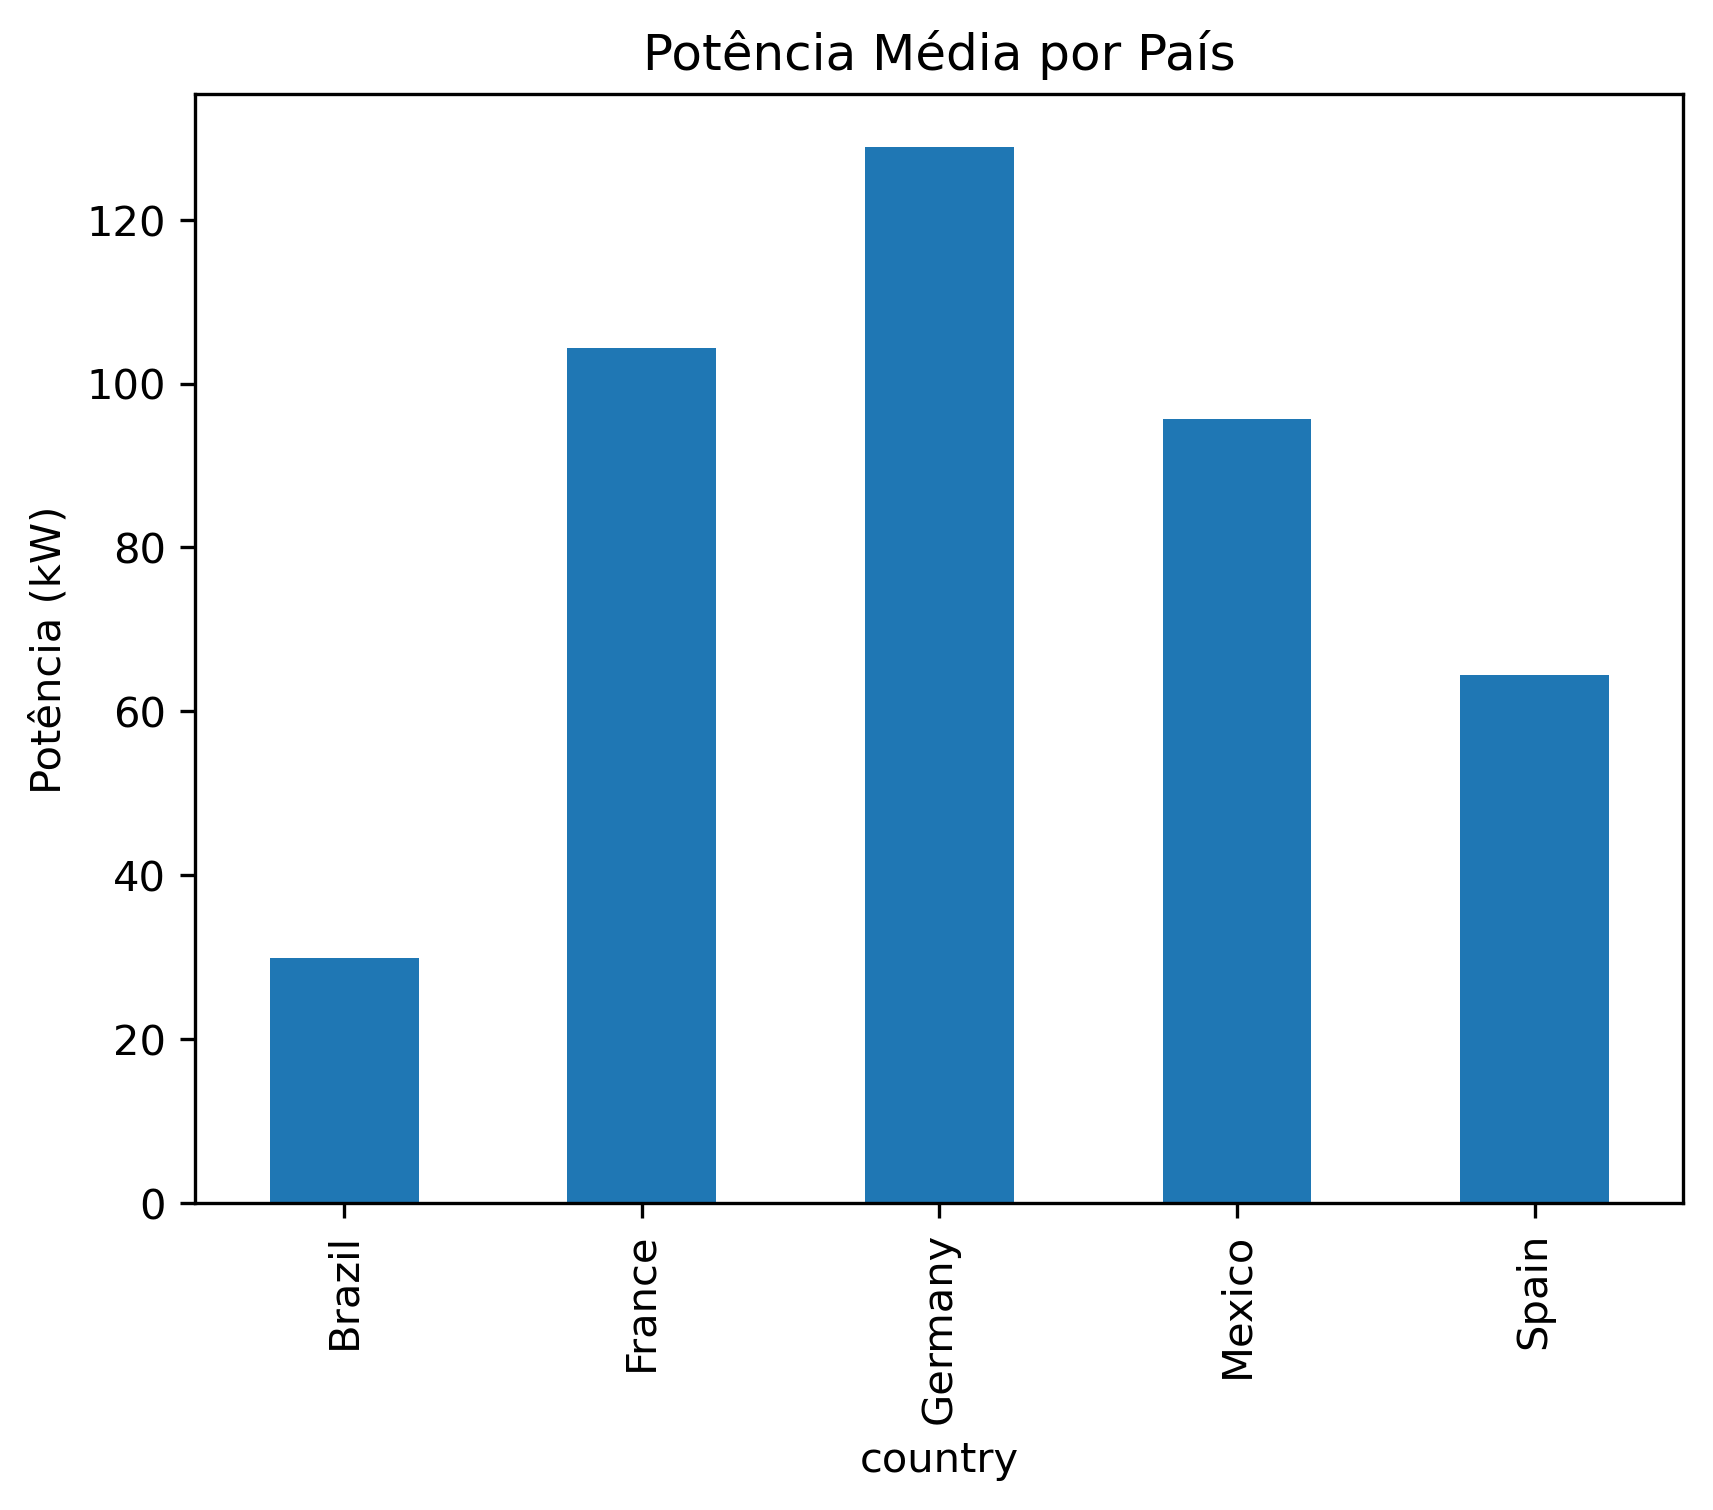
\includegraphics[width=0.8\linewidth]{figures/avg_power_country.png}
\caption{Média de potência de carregamento por país}
\label{fig:avg_power_country}
\end{figure}


\section{Conclusão}
A infraestrutura de recarga de veículos elétricos deve ser analisada como sistema estratégico de integração tecnológica, industrial e regulatória. Os resultados demonstram que a escolha do padrão de conectores afeta diretamente a potência instalada, a eficiência do investimento e a capacidade de expansão da mobilidade elétrica. 

O Brasil apresenta alinhamento tecnológico com o padrão europeu, especialmente pela predominância de CCS2 e Type 2, porém ainda mantém defasagem em potência média instalada quando comparado aos principais benchmarks europeus. 

A consolidação regulatória, a expansão de fast charging e a redução da fragmentação tecnológica representam fatores centrais para o avanço do setor. 

Como continuidade da pesquisa, recomenda-se incorporar análise longitudinal, dados operacionais de utilização e modelos de viabilidade econômica para implantação de infraestrutura em ambientes públicos e privados. 

\end{document}